\documentclass[aspectratio=169]{beamer}

\usepackage[utf8]{inputenc}
\usepackage{array}
\usepackage{booktabs}
\usepackage{bold-extra}
\usepackage{graphics}
\usepackage{hyperref}
\hypersetup{%
  colorlinks=true,
  linkcolor=blue,
  filecolor=blue,
  urlcolor=cyan,
}
\usepackage{listings}
\usepackage{multicol}
\usepackage[absolute,overlay]{textpos}
\usepackage{setspace}
\usepackage{verbatim}
\usepackage{fancyvrb} % for verbatim centering

\usetheme{Warsaw}
\usecolortheme{beaver}
\definecolor{clOrange}{HTML}{E76600}
\definecolor{clAlmostWhite}{HTML}{FEFFD9}
\definecolor{clGreen}{HTML}{007F00}
\definecolor{clFlag}{HTML}{D33682}
\definecolor{clFlagOpt}{HTML}{CB4B16}
\definecolor{clRedFlag}{HTML}{DC322F}
\definecolor{clViolet}{HTML}{4c0070}

\definecolor{clCodeBlue}{rgb}{0.0, 0.18, 0.38}
\definecolor{clCodeGreen}{rgb}{0.0, 0.27, 0.15}
\definecolor{clCodeRed}{rgb}{0.63, 0.0, 0.0}

\title[LTN08 :: PerfectForwarding]{Understanding perfect forwarding and universal references}
\author{Adam Graliński}
\date[FFFE\_21]{\textbf{C++ {\color{red}F}{\color{blue}F}{\color{green}F}{\color{yellow}E}, September 2021}}

\setbeamertemplate{navigation symbols}{}
\setbeamercolor{title}{fg=black}
\setbeamercolor{author}{fg=clAlmostWhite}
\setbeamercolor{date}{fg=clAlmostWhite}
\setbeamerfont{author}{size=\huge}
\setbeamerfont{date}{size=\Large}

\newcommand{\greenemph}[1]{\textit{\textcolor{clGreen}{#1}}}
\newcommand{\cppmethod}[1]{\texttt{\textbf{\textcolor{clCodeBlue}{#1}}}}

\lstset{
  language=C++,
  basicstyle=\ttfamily,
  keywordstyle=\color{clCodeBlue}\ttfamily,
  stringstyle=\color{clCodeGreen}\ttfamily,
  commentstyle=\color{clCodeRed}\ttfamily,
  morecomment=[l][\color{magenta}]{\#}
}

\begin{document}

{\usebackgroundtemplate{%
 
\includegraphics[width=\paperwidth,height=\paperheight]{../common/bg_galaxy.jpg}}
\begin{frame}
\titlepage{}
\end{frame}
}

\begin{frame}
\frametitle{Perfect forwarding problem}
\begin{itemize}
  \item{when a function template forwards its arguments...}
  \begin{itemize}
    \item{...\greenemph{without changing their lvalue/rvalue aspect}}
  \end{itemize}
  \item{impossible before C++11}
  \vspace{1cm}
  \item{\url{https://en.cppreference.com/w/cpp/utility/forward}}
  \item{\url{https://www.modernescpp.com/index.php/perfect-forwarding}}
\end{itemize}
\end{frame}

\begin{frame}
\frametitle{Perfect factory method}
A great concept from \url{https://www.modernescpp.com/index.php/perfect-forwarding} \\
\vspace{2em}
Task: Let's write a function that:
\begin{itemize}
  \item{Can take any number of arguments}
  \item{Will accept both lvalues and rvalues}
  \item{Forwards these arguments \greenemph{verbatim} to the appropriate constructor}
\end{itemize}
\end{frame}

\begin{frame}[fragile]
\frametitle{Perfect factory: first try}
\begin{columns}
  \begin{column}{0.6\textwidth}
    {\tiny \lstinputlisting{code/forwarding1.cpp}}
  \end{column}
  \begin{column}{0.4\textwidth}
    \begin{itemize}
      \item{Works as expected for lvalues}
      \item{Does not work for rvalues}
      \begin{itemize}
        \item{can not bind an rvalue to a non-const lvalue reference}
      \end{itemize}
    \end{itemize}
  \end{column}
\end{columns}
\end{frame}

\begin{frame}[fragile]
\frametitle{Perfect factory: second try}
\begin{columns}
  \begin{column}{0.6\textwidth}
    {\tiny \lstinputlisting{code/forwarding2.cpp}}
  \end{column}
  \begin{column}{0.4\textwidth}
    \begin{itemize}
      \item{OK, let's overload \texttt{create()} to accept constant lvalue references}
      \item{Works as expected for lvalues}
      \item{Now works for rvalues too}
      \item{\textcolor{clRedFlag}{Non-scalable solution}}
      \item{\textcolor{clRedFlag}{Also, \texttt{arg} is not movable now}}
      \item{Solution: \greenemph{std::forward}}
    \end{itemize}
  \end{column}
\end{columns}
\end{frame}


\begin{frame}[fragile]
\frametitle{Perfect factory: third try}
\begin{columns}
  \begin{column}{0.6\textwidth}
    {\tiny \lstinputlisting{code/forwarding3.cpp}}
  \end{column}
  \begin{column}{0.4\textwidth}
    \begin{itemize}
      \item{As advertised on cppreference.org}
      \item{Works flawlessly...}
      \begin{itemize}
        \item{...for \textcolor{clRedFlag}{one} parameter}
      \end{itemize}
      \item{How about extending this to any number of parameters?}
    \end{itemize}
  \end{column}
\end{columns}
\end{frame}


\begin{frame}[fragile]
\frametitle{Perfect factory: solution (fourth try)}
\begin{columns}
  \begin{column}{0.55\textwidth}
    {\fontsize{3}{4} \lstinputlisting{code/forwarding4.cpp}}
  \end{column}
  \begin{column}{0.45\textwidth}
    \begin{itemize}
      \item{Variadic templates to the rescue}
      \item{Works flawlessly...}
      \begin{itemize}
        \item{...for \textcolor{clGreen}{any} number of parameters}
      \end{itemize}
      \vspace{10em}
    \end{itemize}
  \end{column}
\end{columns}
\end{frame}


\begin{frame}[fragile]
\frametitle{Now for the fun part...}
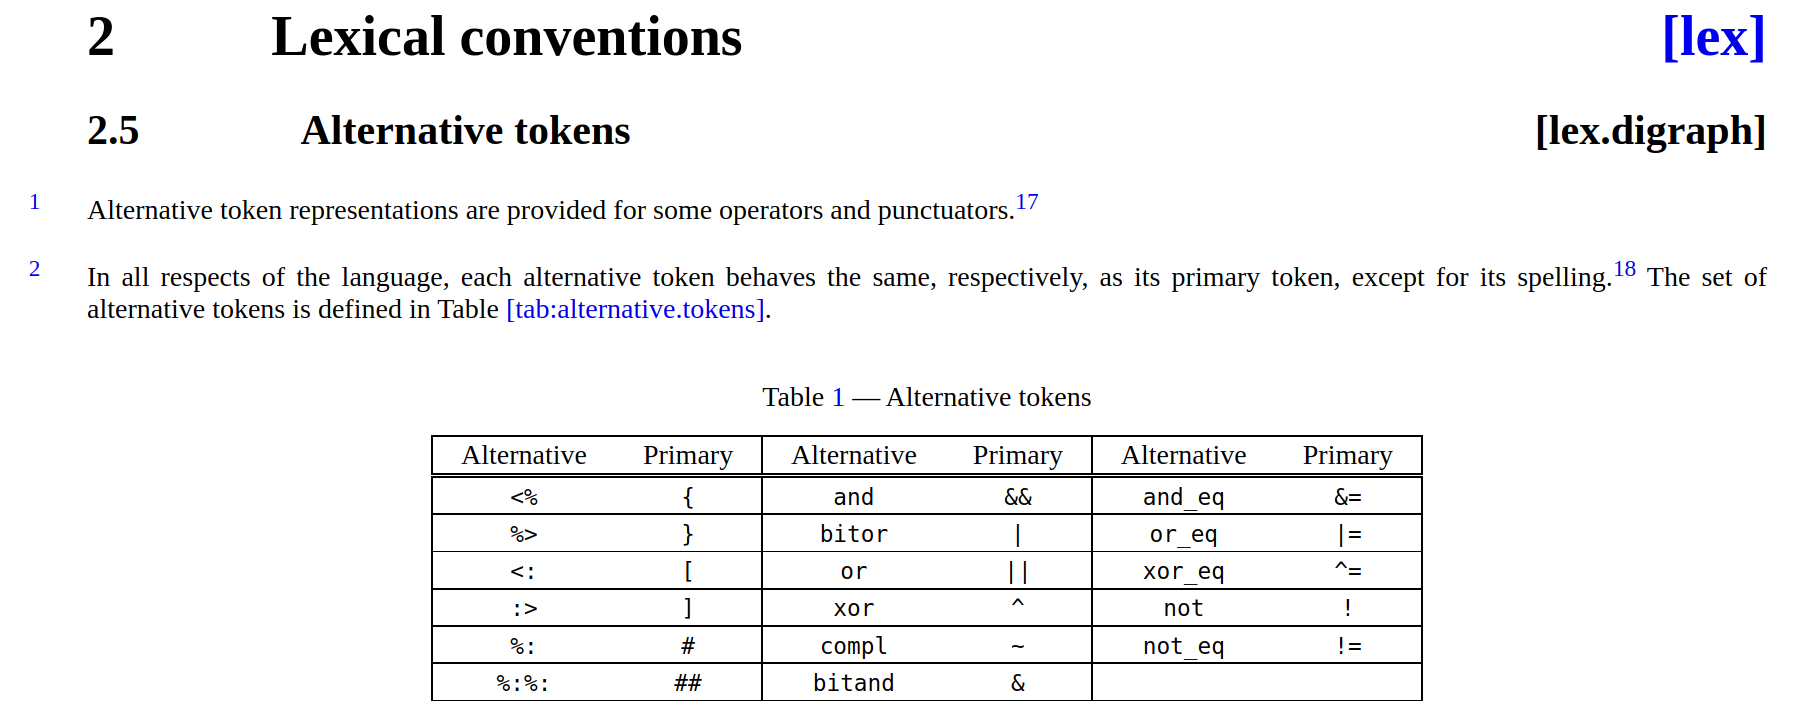
\includegraphics[width=\textwidth]{pics/lexconv.png}
\end{frame}

\begin{frame}[fragile]
\frametitle{Now for the fun part...}
\begin{columns}
  \begin{column}{0.5\textwidth}
    \begin{itemize}
      \item \texttt{auto\&\& fortytwo = 42;}
      \vspace{2em}
      \item \texttt{int const\&\& final}
    \end{itemize}
  \end{column}
  \begin{column}{0.5\textwidth}
    \begin{itemize}
      \item \texttt{auto and fortytwo = 42;}
      \vspace{2em}
      \item \texttt{int const and final}
    \end{itemize}
  \end{column}
\end{columns}
\end{frame}


\begin{frame}[fragile]
\frametitle{Now for the fun part...}
  {\fontsize{3}{4} \lstinputlisting{code/forwarding_galaxybrain.cpp}}
\end{frame}


\begin{frame}
\frametitle{Key takeaways}
{\centering
\begin{itemize}
  \item Perfect forwarding is useful
  \item Lex.digraph is a mess
\end{itemize}

\vspace{2ex}
\begin{center}{\Large Thank you!}\end{center}
}
\end{frame}
\end{document}
